\documentclass{article}
\usepackage{xeCJK}
\usepackage{amsmath}
\usepackage{listings}
\usepackage{xcolor}
\setlength{\parindent}{0pt}
\renewcommand{\baselinestretch}{1.0}
\lstset{
	frame=tb, % draw a frame at the top and bottom of the code block
	showstringspaces=false, % don't mark spaces in strings
	numbers=left, % display line numbers on the left
	commentstyle=\color{green}, % comment color
	keywordstyle=\color{blue}, % keyword color
	stringstyle=\color{red} % string color
}
\usepackage[a4paper,left=20mm,right=20mm,top=15mm,bottom=15mm]{geometry}  

\title{Manacher}
\author{MengChunlei}

\begin{document}
\maketitle
\section{算法目标}
给定字符串$S$. 找到$S$中最长的回文子串. 比如$S$='abaabcd', 则最长的回文子串为'baab'. \par
\section{算法描述}
首先, 回文串的长度可能为奇数也可能为偶数. 为了方便处理, 先将给定的字符串每两个相邻字符中间插入一个原字符串中不存在的字符, 比如'@', 这样最后的最长回文串的长度一定是奇数. 比如处理后上面的字符串为'@a@b@a@a@b@c@d@'. 最长回文串为'@b@a@a@b@', 长度为9. \par
~\\
假设现在$S$是处理后的字符串. 设$S$的长度为$n$. 并且有一个长度为$n$的辅助数组$f$, $f[i]$表示以$S[i]$为中心的回文串的最大半径. \par
~\\
这个算法从前向后依次计算$f[0],f[1],..,f[i-1]$.
~\\~\\
假设$p=max\ \sum_{k=0}^{i-1}(k+f[k]+1)$, 而$c$ 为使得$p$取最大值时对应的$k$. 那么前$i$个位置计算完后的信息如下图所示. \par
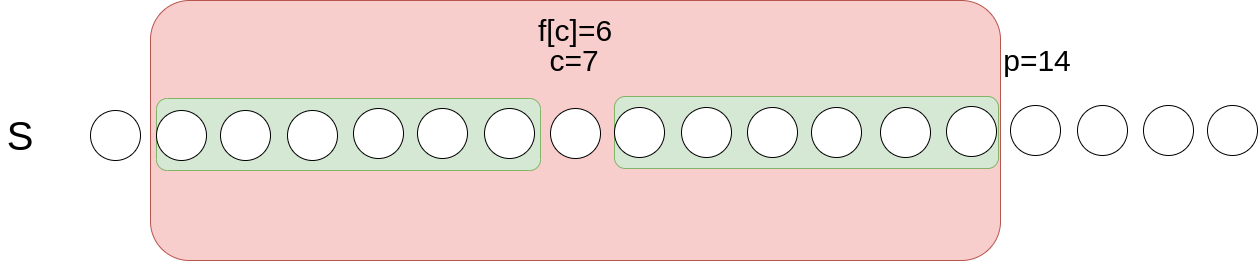
\includegraphics[scale=0.39]{pic1.png} \par
~\\
现在看$f[i]$的计算($c < i\le p$). 分四种情况.\par
~\\
(1) $i= p$: 这时候, 前面的任何信息不能借鉴, 只能从$i$向外, 依次比较两边对称位置的字符, 直到一个数字$x$满足, $S[i+x]\ne S[i-x]$,此时$f[i]=x-1$, 并且更新$c=i,p=i+x$. \par
~\\
(2) $c<i<p$且 $i+f[2c-i]<p-1$: 如下图所示,$2c-i$是$i$关于$c$对称的位置.四个红色方框里面的串相等, 并且$S[7]\ne S[1]$, 且$S[1]=S[13]$,所以$S[7]\ne S[13]$, 此时$f[i]=f[2c-i]=2$\par
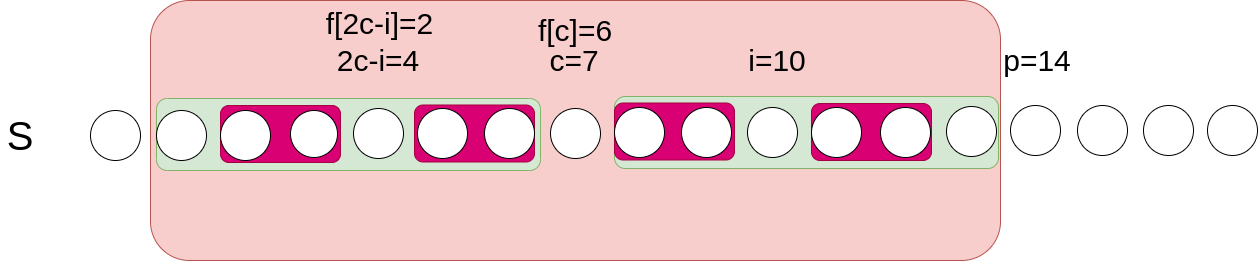
\includegraphics[scale=0.39]{pic2.png} \par
~\\
(3) $c<i<p$且 $i+f[2c-i]= p-1$: 如下图所示, 从已知的信息中, 无法判断$S[14]$跟$S[6]$是否相等. 这时候跟情况(1)一样, 需要扩展检查并更新$c,p$. \par
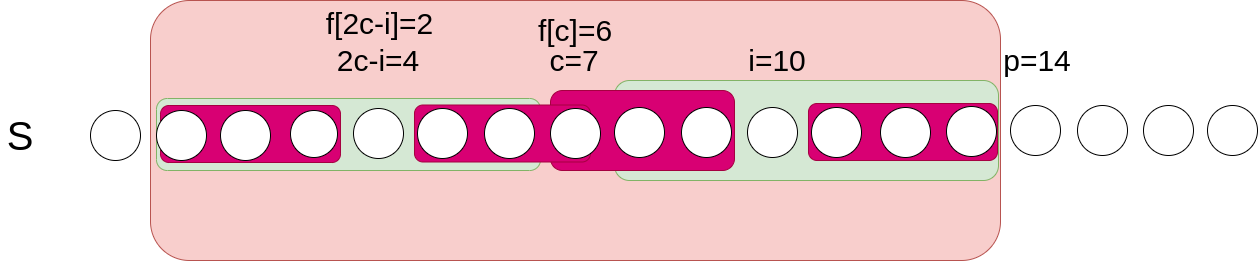
\includegraphics[scale=0.39]{pic3.png} \par
~\\
(4) $c<i<p$且 $i+f[2c-i]> p-1$: 这种情况也跟第一种情况一样, 需要扩展检查. \par
~\\
下面是实现的代码.
\begin{lstlisting}[language=C++, caption={Manacher}]

int Manacher(const std::string &S) {
  int n = static_cast<int>(S.size());
  std::vector<int> f(n);
  int p = -1;
  int c = -1;
  int result = 0;
  for (int i = 0; i < n; ++i) {
    f[i] = i < p ? std::min(f[2 * c - i], p - i - 1) : 0;
    while (i + f[i] + 1 < n && i - f[i] - 1 >= 0) {
      if (S[i - f[i] - 1] == S[i + f[i] + 1]) {
        ++f[i];
      } else {
        break;
      }
    }
    if (i + f[i] + 1 > p) {
      p = i + f[i] + 1;
      c = i;
    }
    result = std::max(result, f[i]);
  }
  return result * 2 + 1;
}
\end{lstlisting}


\end{document}
